\subsubsection{Entry Criteria}
	In order to start a correct integration test we must ensure the following conditions are granted:

	\begin{itemize}
		\item Requirements Analysis and Specification Document as well as the Design Document must be complete in each section and up to date, reflecting the current state of the project
		\item All sub-components must be already unit tested and bug free
		\item Risk Assessment has been layed out since it'll serve us in critical-first module integration
	\end{itemize}

	In addition to this we assume that all algorithms that interface external agents and make use of APIs will be already tested and that they will work as intended in receiving external data when proceeding with integration (we're talking about all sub-components that contain the word 'API' in API Manager component).


\subsubsection{Elements to be integrated}
	All components we created and delimited in components diagram are going to be integrated. All components that give the chance to do so, will also be tested regarding the integration of the single subcomponents.
	\documentclass[12pt, a4paper]{article}

\begin{document}


IMPLEMENTATION:

\begin{itemize}
	\item	 Listener								(API Manager)
	\item API Request Dispatcher		(Travlendar Server)
	\item	 OpenWeatherMap API 			(API Manager)
	\item Google Maps API					(API Manager)
	\item Google Transit API				(API Manager)
	\item CAR2GO API							(API Manager)
	\item Other API-Based system		(API Manager)
	\item DBMS									(Travlendar Server)
	\item Autentication Manager          (Access Manager)
	\item Profile Manager					(Application Aggregator)
	\item User Action Handler				(Application Aggregator)
	\item SignUp Handler 					(Access Manager)
	\item Saved Login Data   				(Access Manager)
	\item Appointment Aggregator		(Calendar Manager)
	\item Preference Handler				(Preference Manager)
	\item Season Pass Handler			(Preference Manager)
	\item Excluded Vehicles List			(Preference Manager)
	\item Preference List						(Preference Manager)
	\item Trip List								(Calendar Manager)
	\item Break List								(Calendar Manager)
	\item Scheduler 							(Travel Logic)
	\item Trip Handler							(Travel Logic)
	\item Payment Handler					(Payment Manager)
	\item Credit Card List					(Payment Manager)
	\item Notification Manager
	\item Localization Manager
	\item Guest View 							(Mobile Application)
	\item User View								(Mobile Application)


\end{itemize}

\end{document}


\subsubsection{Integration Testing Strategy}
	The integration of the system will be guided by a bottom-up approach. This strictly comes from an analysis of the dependency structure of the components diagram provided in the DD, restructured in Figure \ref{DependencyTreehighLevel} and Figure \ref{DependencyTreeComplete} to better highlight the key modules and their connections.
	
	\begin{figure}[H]
		\centering
		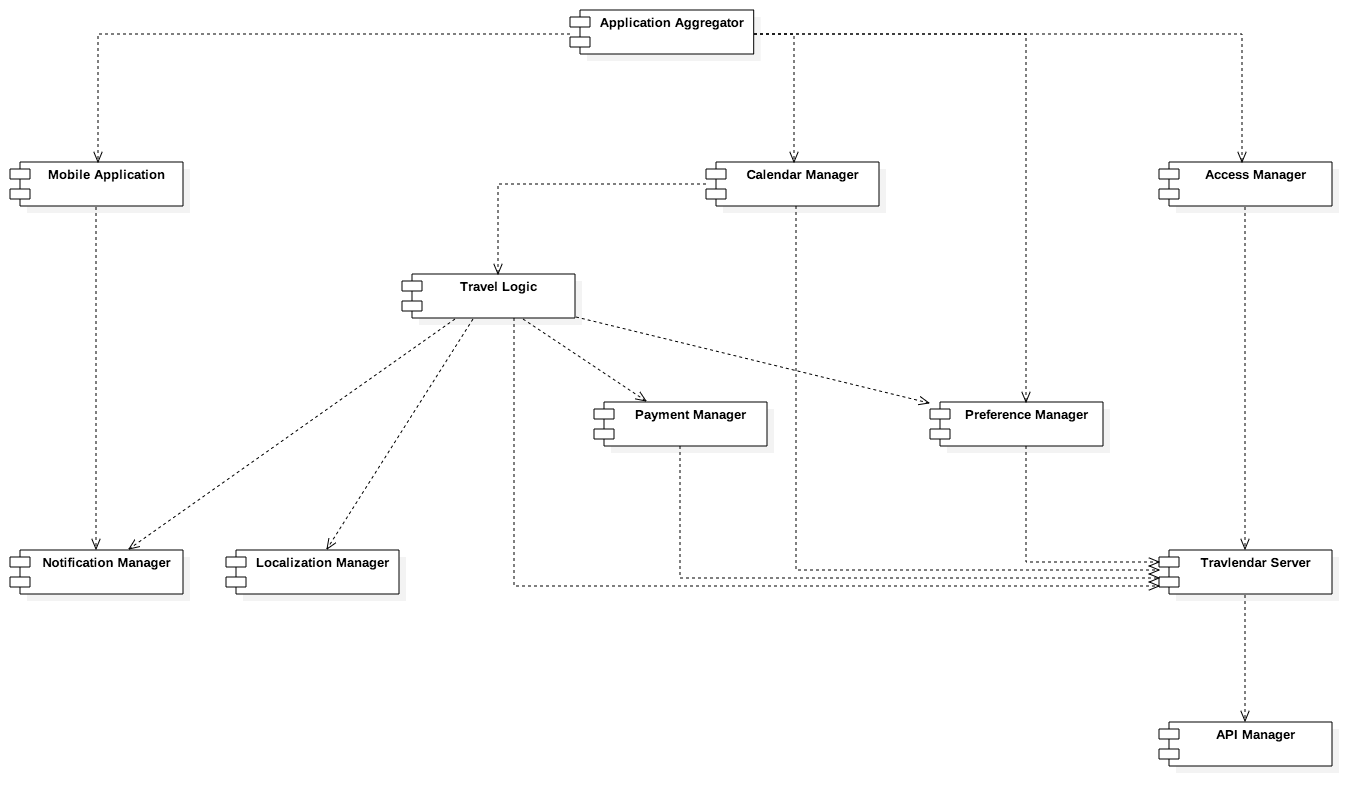
\includegraphics[width=0.9\textwidth]{dependencyTree/dependencyTreeComponent}
		\caption{Dependency tree of components: high level view.}
		\label{DependencyTreehighLevel}
	\end{figure}
	
	\vfill
	
	\begin{figure}[H]
		\centering
		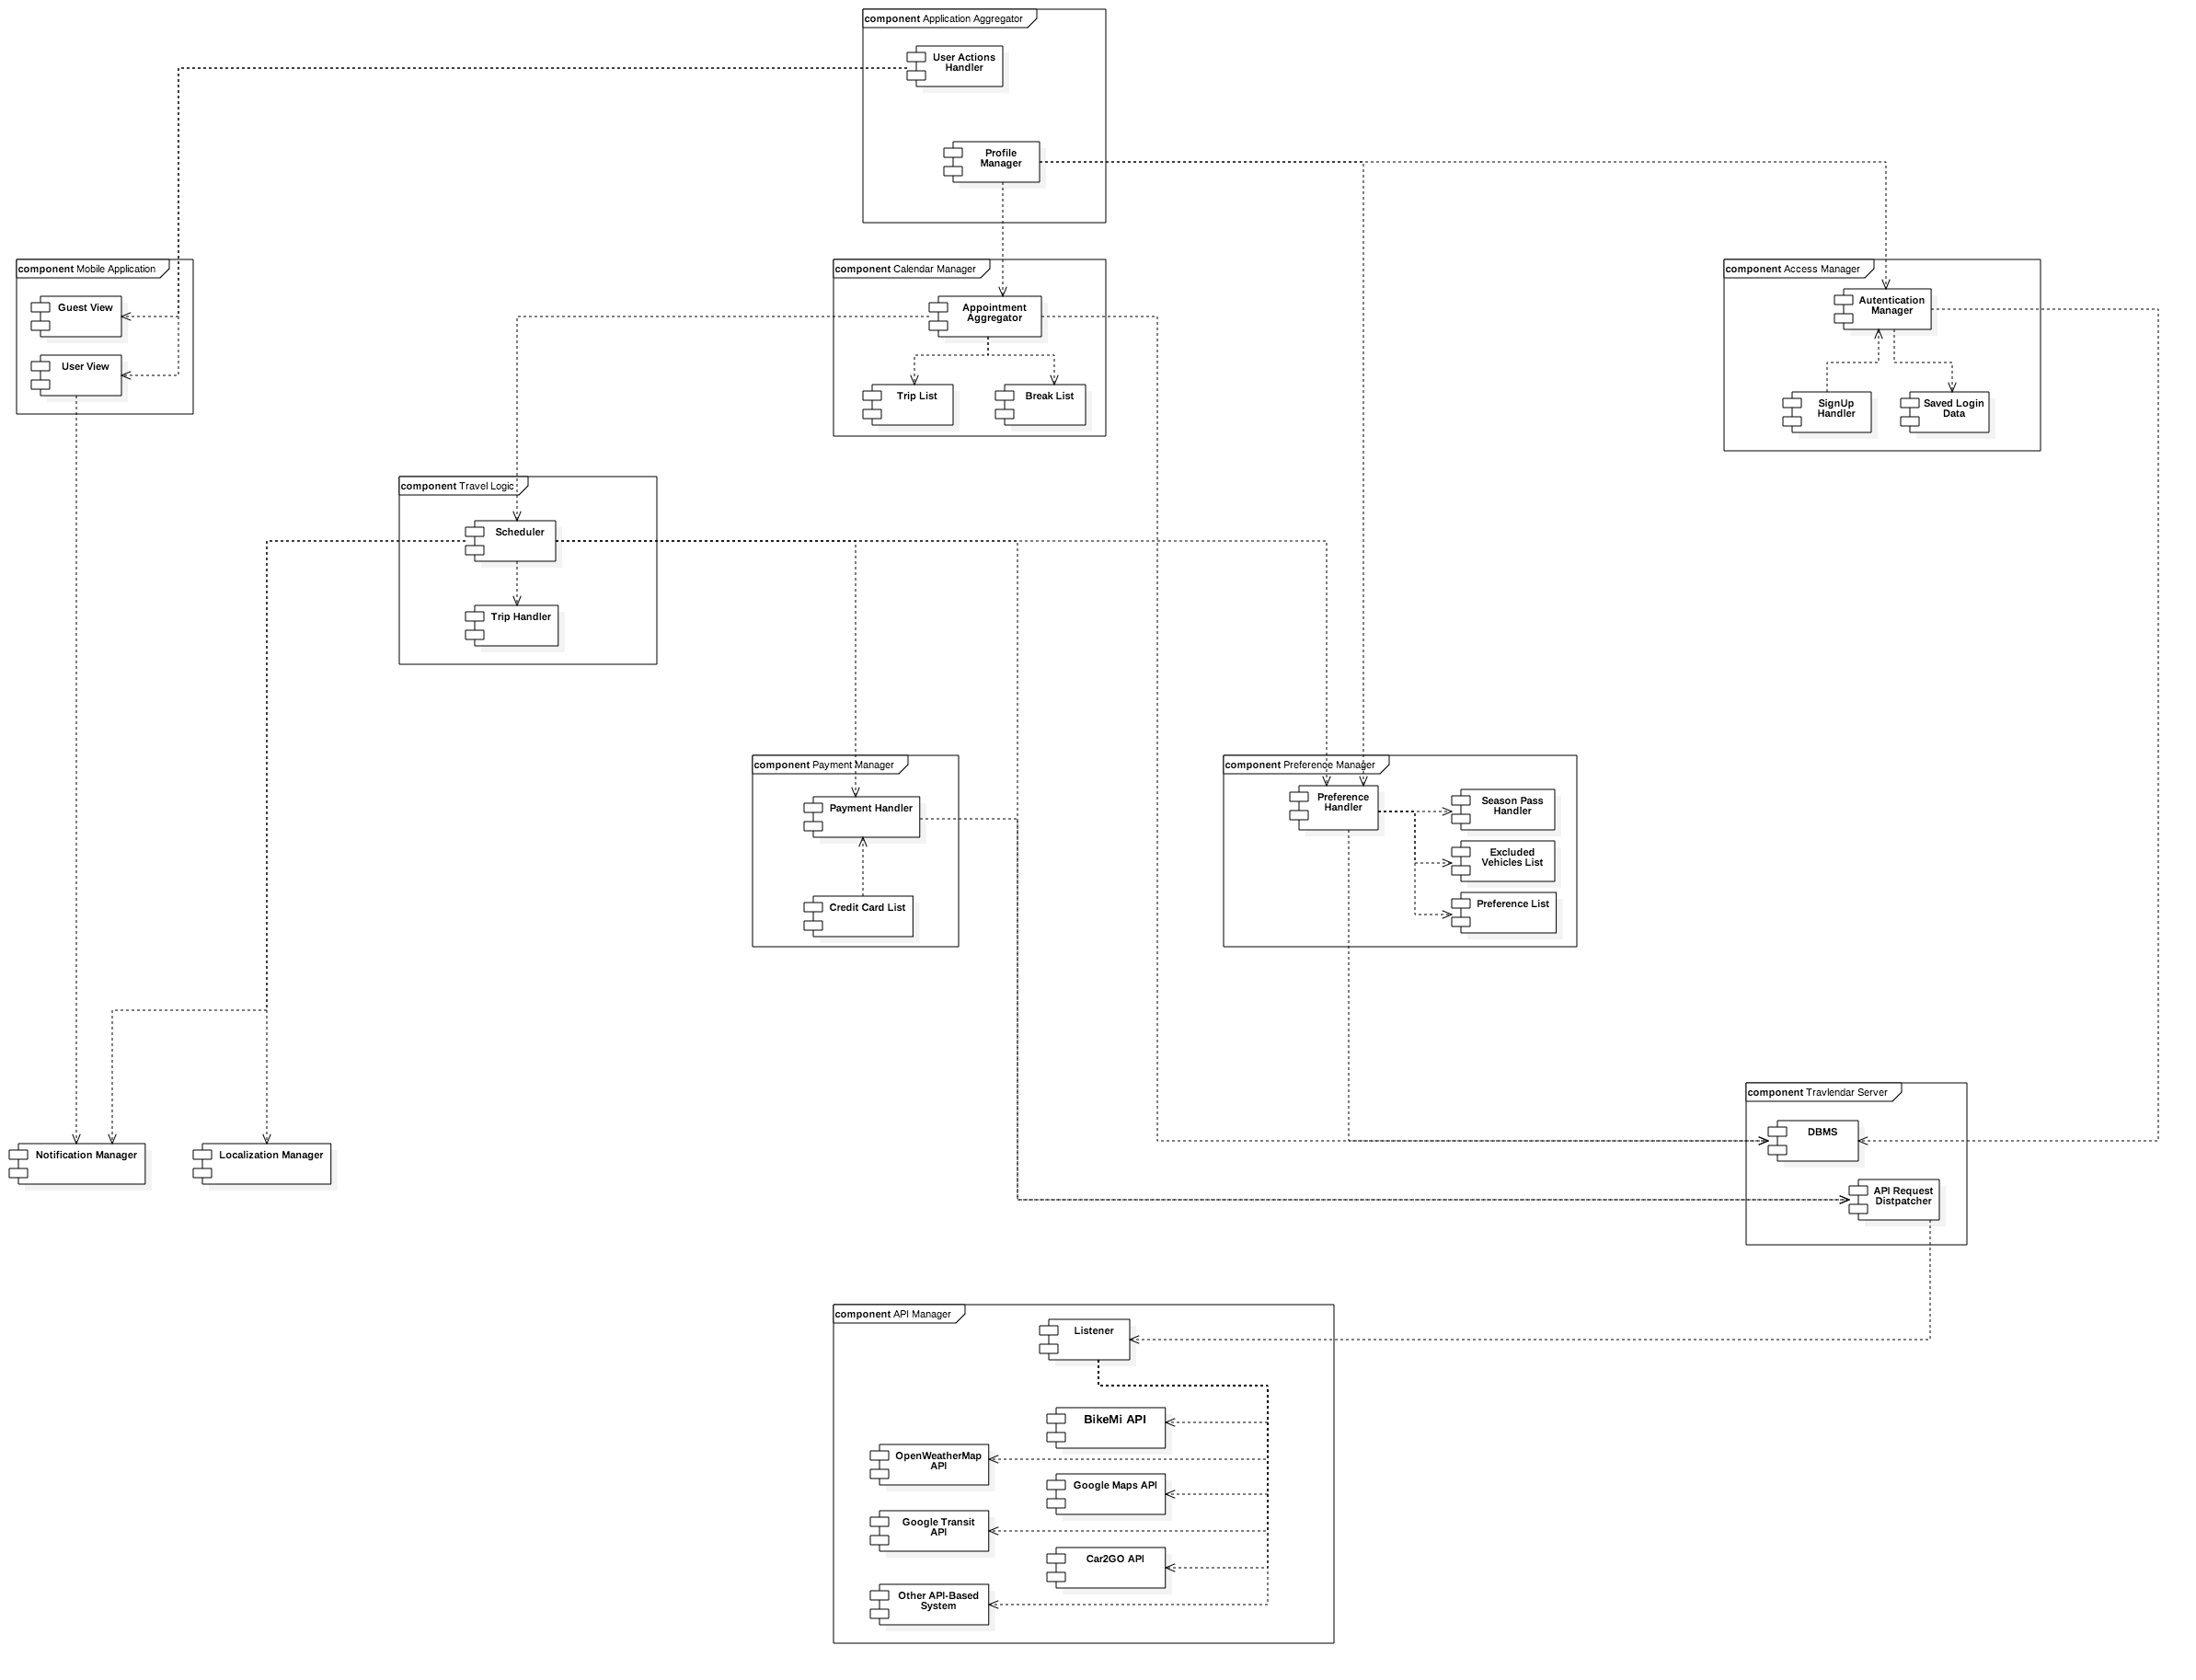
\includegraphics[width=0.9\textwidth]{dependencyTree/dependencyTreeSubcomponents}
		\caption{Dependency tree of components: complete system view.}
		\label{DependencyTreeComplete}
	\end{figure}

\subsubsection{Sequence of component integration}
	From a component perspective we can safely say we adopted a bottom-up policy for the integration plan, while we also used a critical-first approach in sub-components integration (requiring, therefore, stubs in such cases). 
	Our choice has mainly been driven by its ease and by the relatively small scale of our system.
	
	Sequence of component/function integration.
	It's time for us to detail the integration order of our components, delving in what we simply anticipated with our dependency diagrams.
	\begin{description}
	\item[Component]: API Manager.\\
		\textit{Internal integration strategy}: Bottom - Up.\\
		\textit{Integration order}:
		\begin{itemize}
			\item[-] Google Maps API.
			\item[-] OpenWeatherMap.
			\item[-] Google Transit API.
			\item[-] Car2Go API.
			\item[-] BikeMi API.
			\item[-] Other API-Based System.
			\item[-] Listener.
		\end{itemize}
		
		\begin{figure}[H]
			\centering
			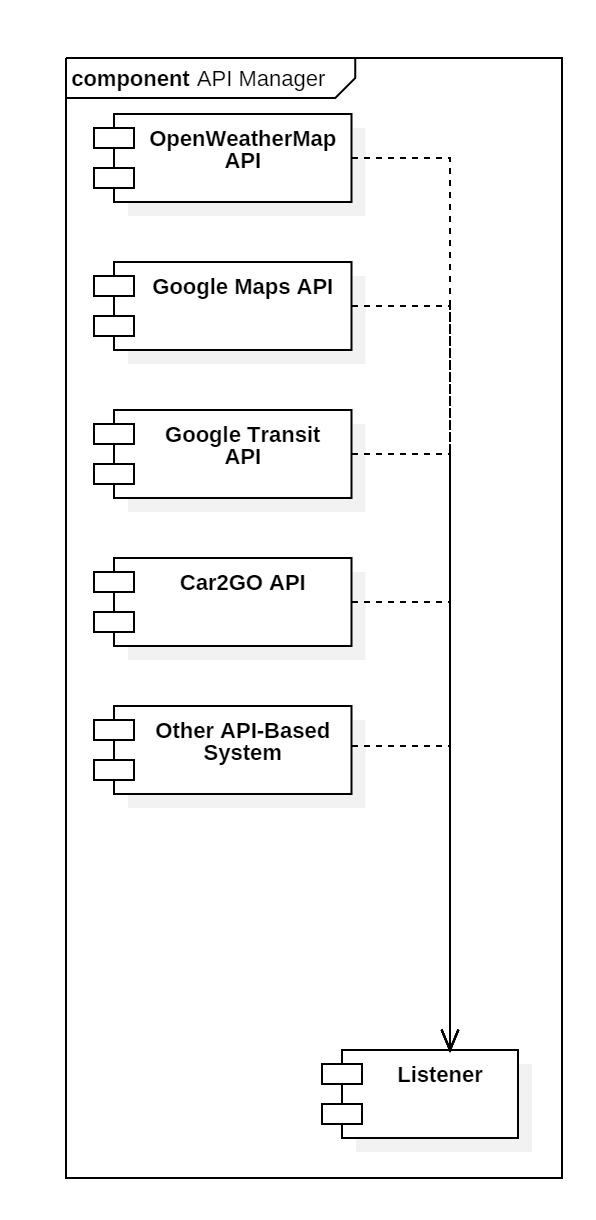
\includegraphics[width=0.5\textwidth]{IntegrationPlan/APIManager}
		\end{figure}
		
		
	\vskip1.5cm
	\item[Component]: Travlendar Server.\\
		\textit{Internal integration strategy}: Critical - First.\\
		\textit{Integration order}:
		\begin{itemize}
			\item[-] DBMS.
			\item[-] API Request Dispatcher.
		\end{itemize}
		
		\begin{figure}[H]
			\centering
			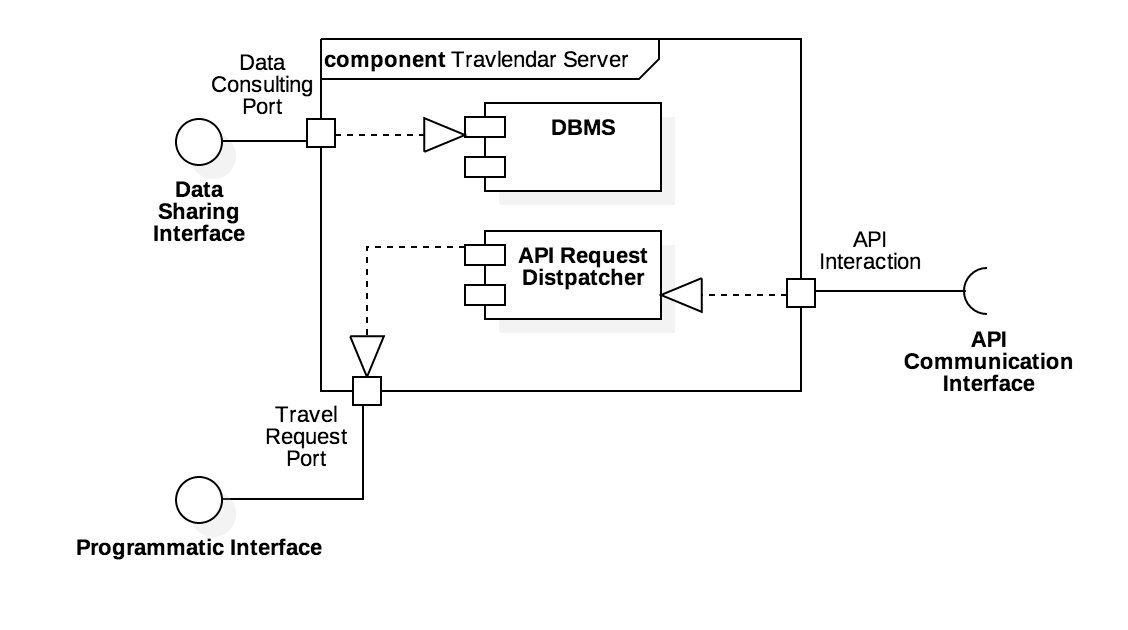
\includegraphics[width=0.5\textwidth]{IntegrationPlan/travlendarServer}
		\end{figure}
	
	
	\vskip1.5cm
	\item[Component]: Localization Manager doesn't need sub-components integration plan.

	\vskip1.5cm
	\item[Component]: Notification Manager doesn't need sub-components integration plan.
	
	\vskip1.5cm
	\item[Component]: Payment Manager.\\
		\textit{Internal integration strategy}: Bottom - Up.\\
		\textit{Integration order}:
		\begin{itemize}
			\item[-] Payment Handler.
			\item[-] Purchase History.
		\end{itemize}
		
		\begin{figure}[H]
			\centering
			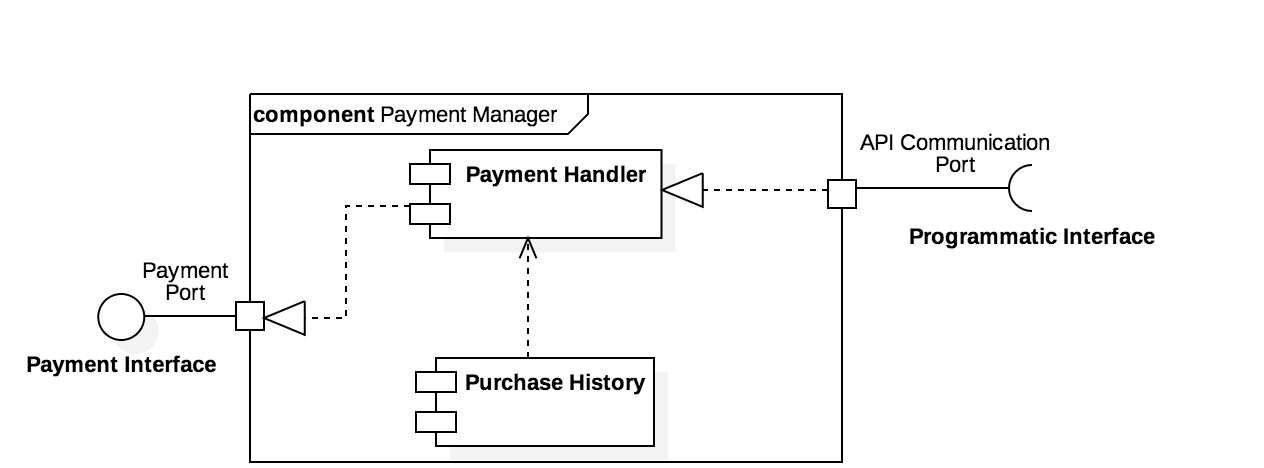
\includegraphics[width=0.5\textwidth]{IntegrationPlan/paymentManager}
		\end{figure}
	
	
	\vskip1.5cm
	\item[Component]: Preference Manager.\\
		\textit{Internal integration strategy}: Bottom - Up\\
		\textit{Integration order}:
		\begin{itemize}
			\item[-] Excluded Vehicles List.
			\item[-] Season Pass Handler.
			\item[-] Preferences List.
			\item[-] Preference Handler.
		\end{itemize}
		
		\begin{figure}[H]
			\centering
			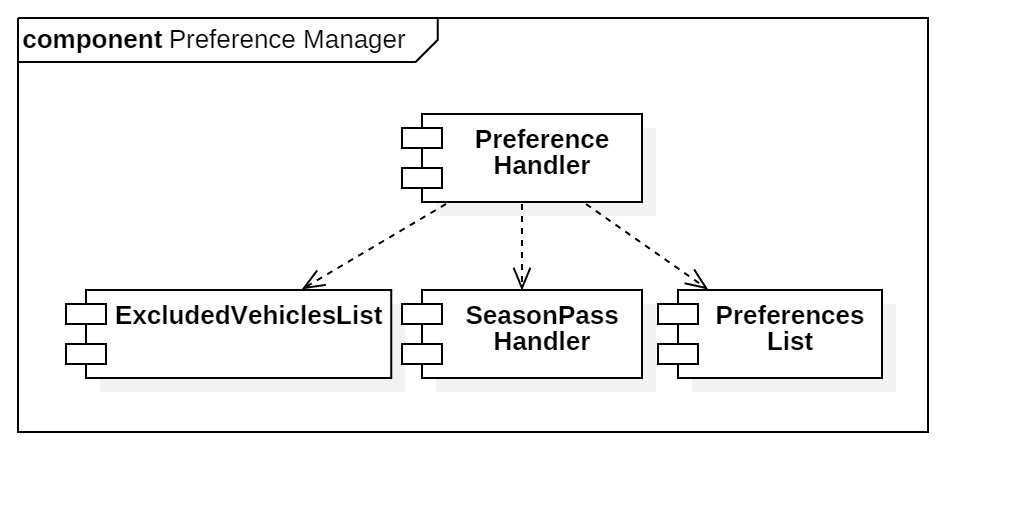
\includegraphics[width=0.5\textwidth]{IntegrationPlan/preferenceManager}
		\end{figure}
		
		
	\vskip1.5cm
	\item[Component]: Travel Logic.\\
		\textit{Internal integration strategy}: Bottom - Up.\\
		\textit{Integration order}:
		\begin{itemize}	
			\item[-] Trip Handler.
			\item[-] Scheduler.
		\end{itemize}
		
		\begin{figure}[H]
			\centering
			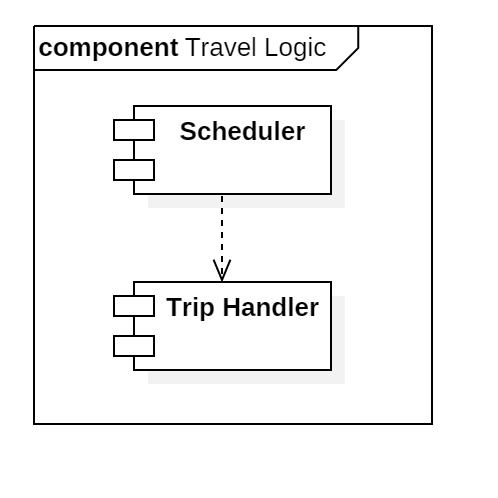
\includegraphics[width=0.5\textwidth]{IntegrationPlan/travelLogic}
		\end{figure}
		
		
	
	\vskip1.5cm
	\item[Component]: Mobile Application.\\
		\textit{Internal integration strategy}: Critical - First.\\
		\textit{Integration order}:
		\begin{itemize}
			\item[-] User View.
			\item[-] Guest View.
		\end{itemize}
		
		\begin{figure}[H]
			\centering
			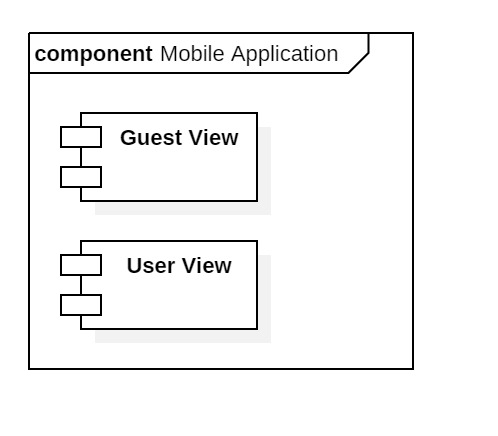
\includegraphics[width=0.5\textwidth]{IntegrationPlan/mobileApplication}
		\end{figure}
	
	
	
	\vskip1.5cm
	\item[Component]: Calendar Manager.\\
		\textit{Internal integration strategy}: Bottom - Up.\\
		\textit{Integration order}:
		\begin{itemize}
			\item[-] Trip List.
			\item[-] Break List.
			\item[-] Appointment Aggregator.
		\end{itemize}
		
		\begin{figure}[H]
			\centering
			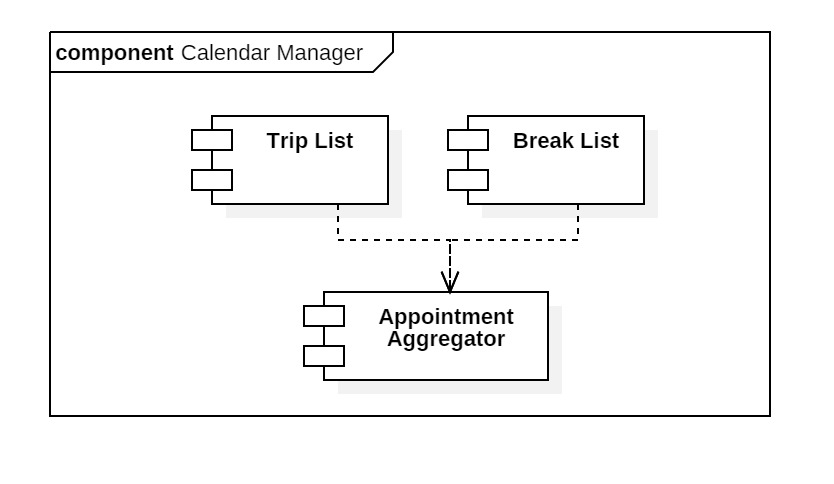
\includegraphics[width=0.5\textwidth]{IntegrationPlan/calendarManager}
		\end{figure}


	\vskip1.5cm
	\item[Component]: Access Manager.\\
		\textit{Internal integration strategy}: Critical - first.\\
		\textit{Integration order}:
		\begin{itemize}
			\item[-] Authentication Manager.
			\item[-] SignUp Handler.
			\item[-] Saved Login Data.
		\end{itemize}
		
		\begin{figure}[H]
			\centering
			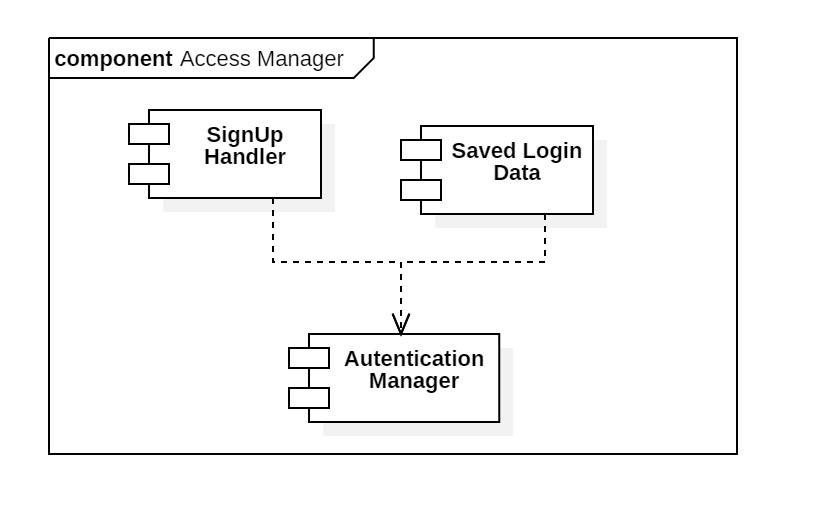
\includegraphics[width=0.5\textwidth]{IntegrationPlan/accessManager}
		\end{figure}
		
		
	\vskip1.5cm
	\item[Component]: Application Aggregator.\\
		\textit{Internal integration strategy}: Critical-First.\\
		\textit{Integration order}:
		\begin{itemize}
			\item[-] Profile Manager.
			\item[-] User Actions Handler.
		\end{itemize}
		
		\begin{figure}[H]
			\centering
			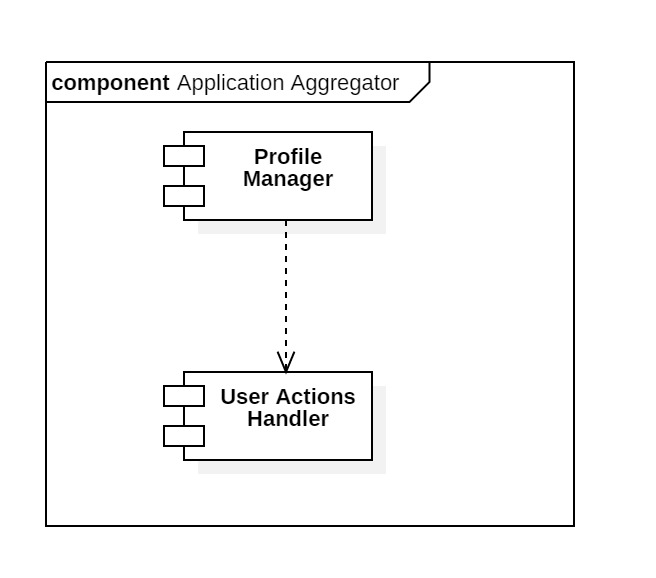
\includegraphics[width=0.5\textwidth]{IntegrationPlan/applicationAggregator}
		\end{figure}
		
\end{description}
	

\vfill
\subsubsection{Subsystem integration sequence}
	The integration of the macro-components is performed, as said, in a bottom-up fashion. Below are the 6 steps in which this process has been divided for scheduling reasons.
	Inside a single step, multiple macro-components participate in the integration, each one relying on the macro-components in the previous levels.
	
	\begin{description}
	
	\item Step 1		
		\begin{figure}[H]
			\centering
			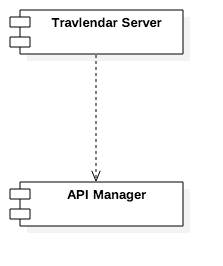
\includegraphics[width=0.25\textwidth]{componentIntegrationStepByStep/step1}
			\caption{Subsystem integration sequence: step 1.}
		\end{figure}
	
	\vfill
	\item Step 2
		\begin{figure}[H]
			\centering
			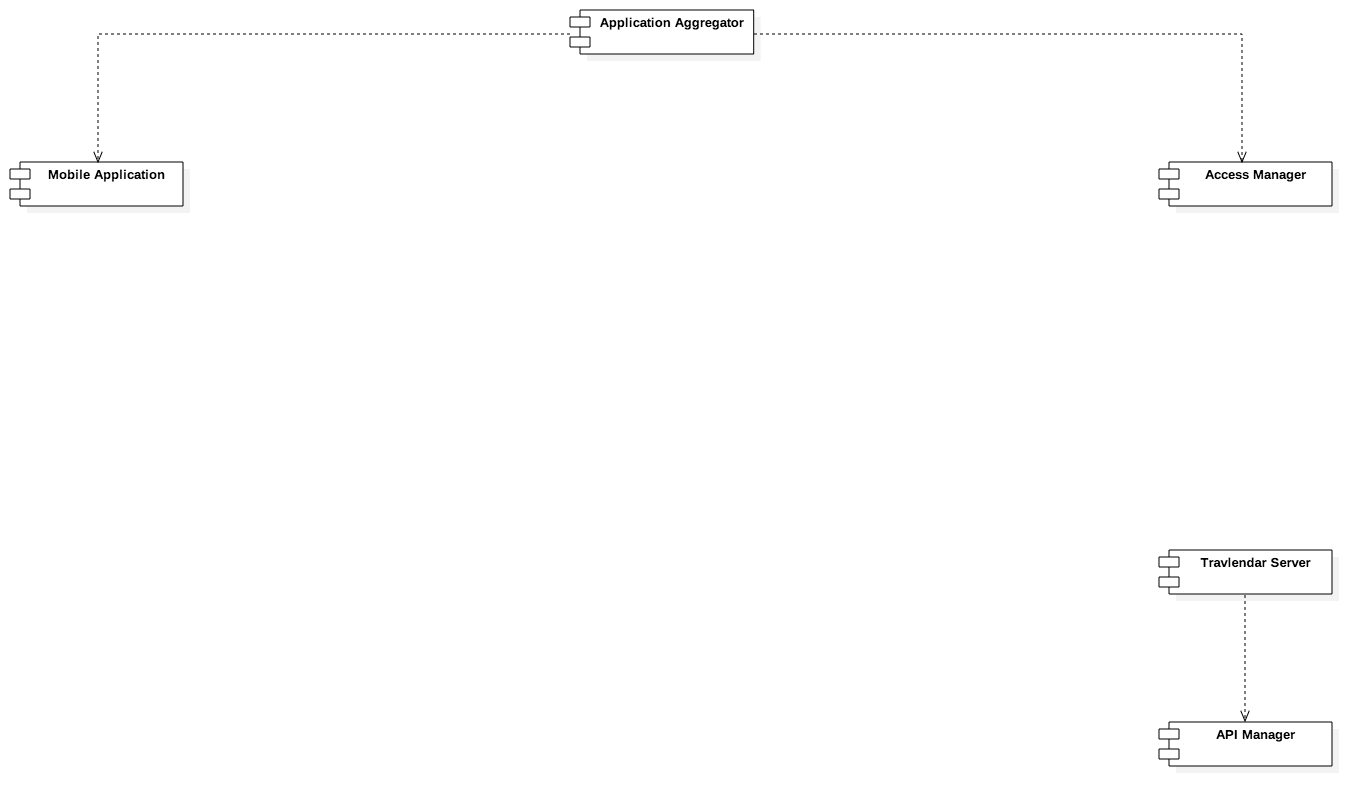
\includegraphics[width=0.95\textwidth]{componentIntegrationStepByStep/step2}
			\caption{Subsystem integration sequence: step 2.}
		\end{figure}
	
	\bigskip
	\item Step 3
		\begin{figure}[H]
			\centering
			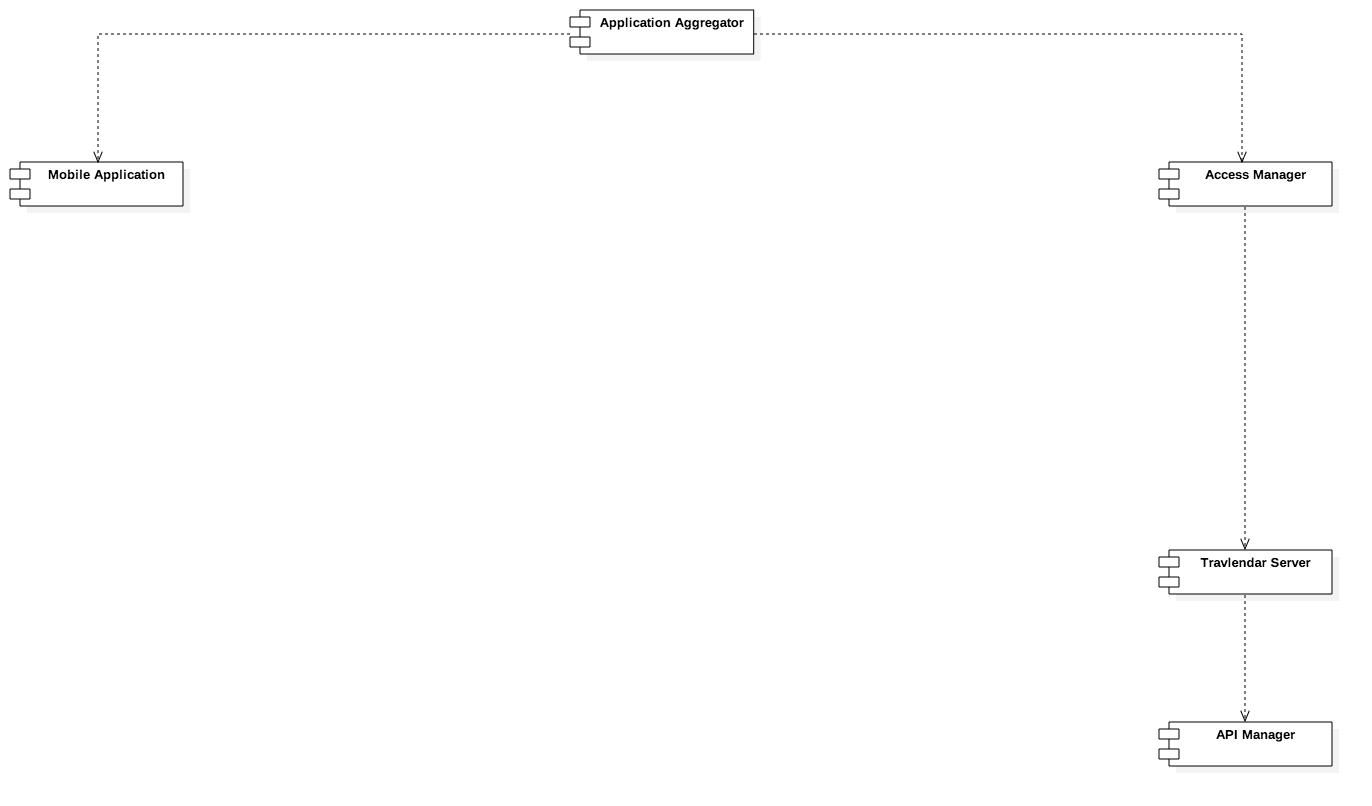
\includegraphics[width=0.95\textwidth]{componentIntegrationStepByStep/step3}
			\caption{Subsystem integration sequence: step 3.}
		\end{figure}
		
	\bigskip
	\item Step 4
		\begin{figure}[H]
			\centering
			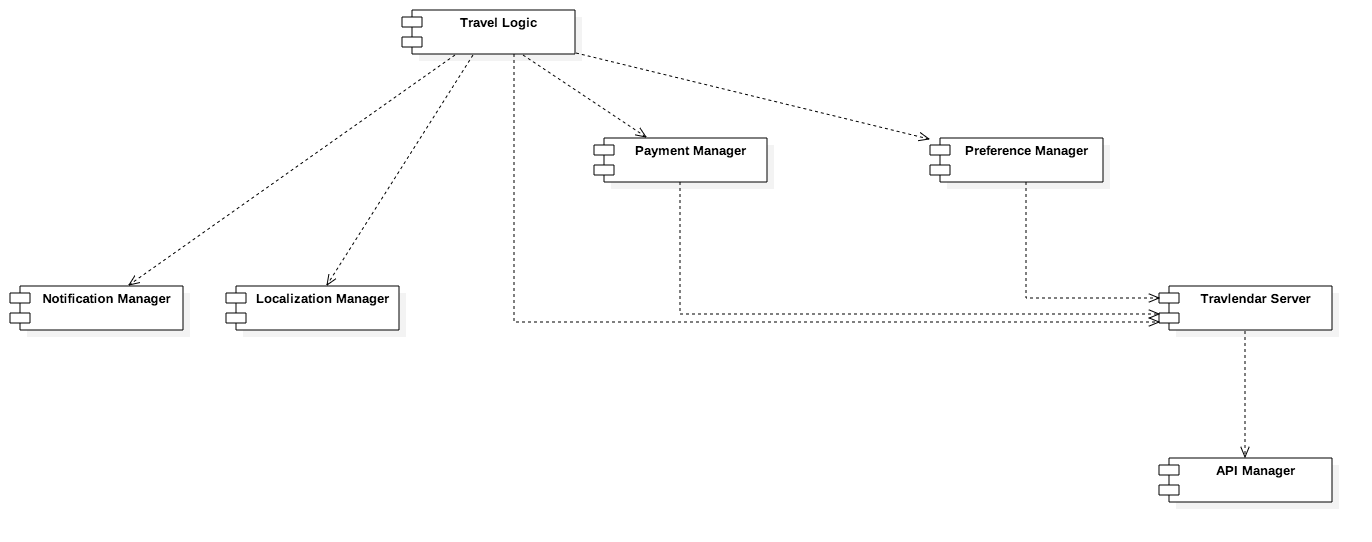
\includegraphics[width=0.95\textwidth]{componentIntegrationStepByStep/step4}
			\caption{Subsystem integration sequence: step 4.}
		\end{figure}
		
	\bigskip
	\item Step 5
		\begin{figure}[H]
			\centering
			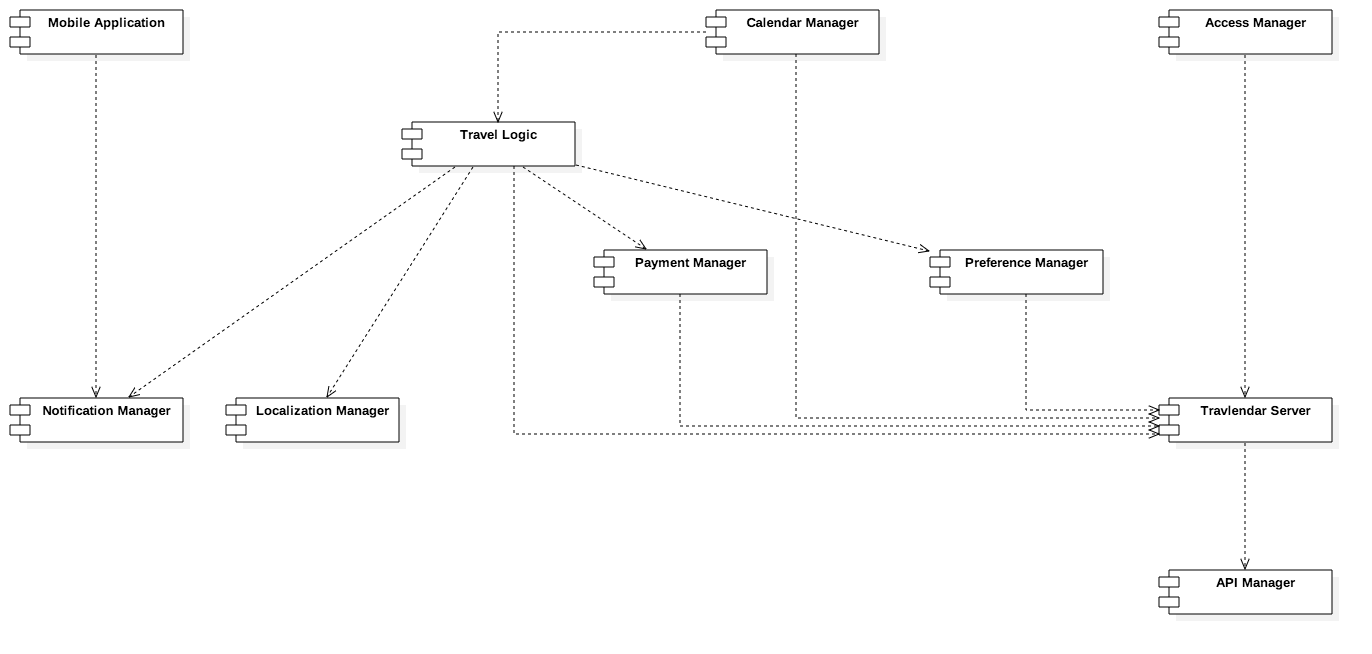
\includegraphics[width=0.95\textwidth]{componentIntegrationStepByStep/step5}
			\caption{Subsystem integration sequence: step 5.}
		\end{figure}
		
	\bigskip	
	\item Step 6
		\begin{figure}[H]
			\centering
			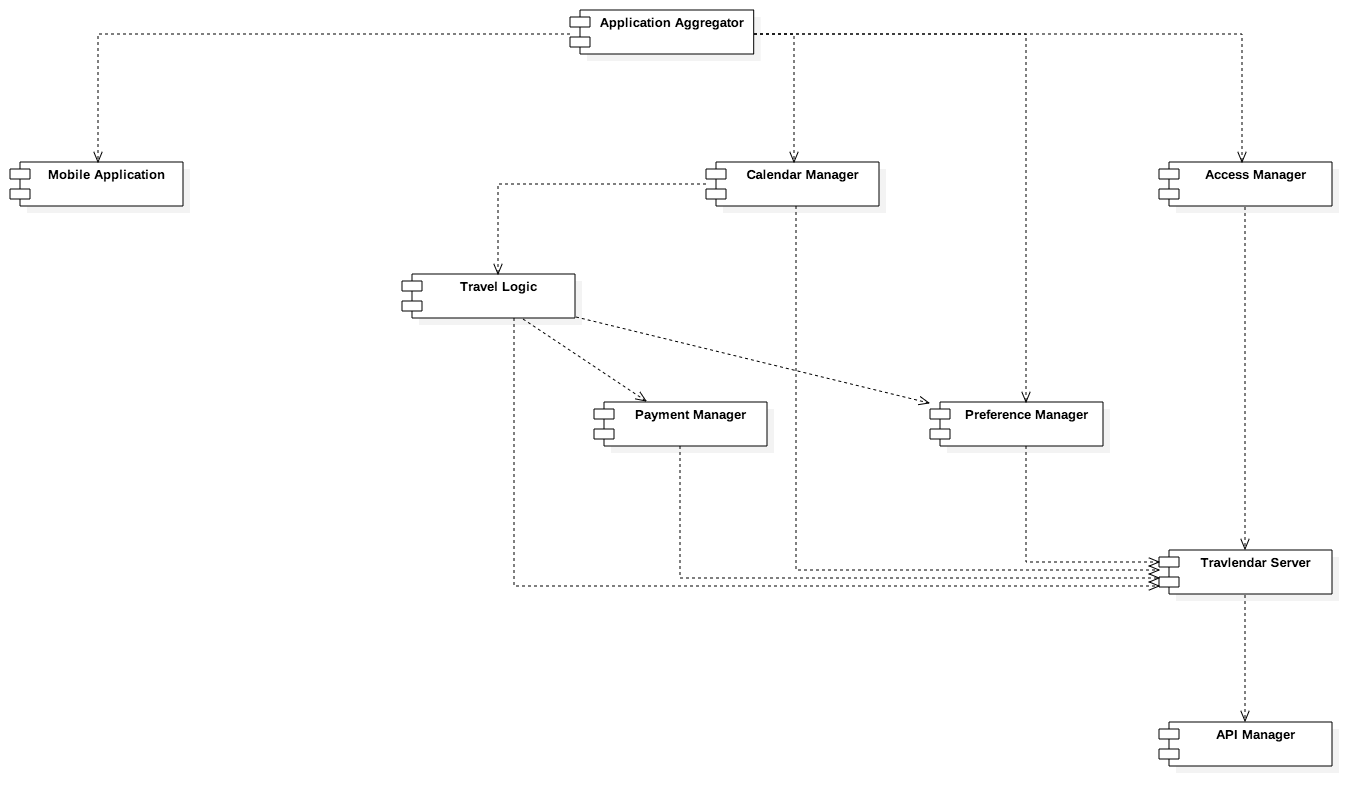
\includegraphics[width=0.95\textwidth]{componentIntegrationStepByStep/step6}
			\caption{Subsystem integration sequence: step 6.}
		\end{figure}

	\end{description}
	
